\documentclass[../main.tex]{subfiles}
\graphicspath{{\subfix{../figures/}}}
%
\begin{document}
\section{适配器模式(Adapter)}
%
\textbf{结构模式}描述如何将类或者对象组织在一起形成特定的结构,以实现更为复杂、强大的功能。结构模式可以分为:
\begin{itemize}
  \item 类的结构模式:使用继承来把类、接口等组合起来,以形成更大的结构。类的结构模式是静态的。典型例子是类形式的适配器模式。
  \item 对象的结构模式:描述怎样把各种不同类型的对象组合在一起,以实现新的功能的方法。对象的结构模式是动态的。
    典型的结构模式有代理模式,其它包括合成模式、享元模式、装饰模式、对象形式的适配器模式。
\end{itemize}
%
\textbf{适配器模式}(Adapter Pattern)把一个类的接口变换成客户端所需要的另一种接口,
从而使原本因接口不匹配而无法在一起工作的两个类能够在一起工作。

\textbf{名称的由来}:这很像变压器,
变压器把一种电压变换成另一种电压。把美国的电器拿回中国大陆来用的时候,
用户就面临电压不同的问题。美国的生活用电电压是110v,而中国的电压是220v。
如果要在中国使用美国的电器,就必须有一个能把220v电压转换成110v电压的变压器。
而这就像是本模式所做的事,因此此模式也常常被称为变压器模式.

\textbf{适配器模式的两种形式}:
适配器模式有类的适配器模式和对象的适配器模式两种不同的形式。如下图所示,左边是类的适配器模式,右边是对象的适配器模式。
\begin{figure}[H]
  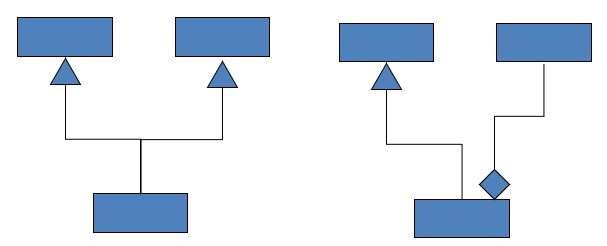
\includegraphics[width=0.40\textwidth]{20_1.jpg}
\end{figure}
%
\subsection{类的适配器模式的结构}
类的适配器模式把被适配的类的API转换成为目标类的API,其静态结构图如下图所示。
%
\begin{figure}[H]
  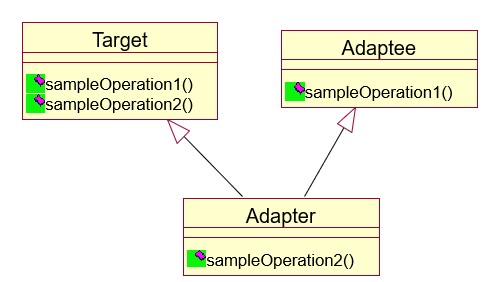
\includegraphics[width=0.50\textwidth]{20_2.jpg}
\end{figure}
%
Adaptee类没有提供sampleOperation2()方法,而客户端则需要使用这个方法。
为使客户端能够使用Adaptee类,提供一个中间环节,即类Adapter,把Adaptee的API与Target类的API衔接起来。

\textbf{模式所涉及的角色有}:
\begin{itemize}
  \item 目标(Target)角色:这就是所期待得到的接口。
  \item 源(Adaptee)角色:现有需要适配的接口。
  \item 适配器(Adapter)角色:适配器类是本模式的核心。
    适配器把源接口转换成目标接口。显然,这一角色不可以是接口,而必须是具体类。
\end{itemize}
%
\begin{lstlisting}[language=java]
public interface Target {
  void sampleOperation1();  //源类的方法
  void sampleOperation2();  //源类没有的方法
}

public class Adaptee {
  public void sampleOperation1() {  }
}

public class Adapter extends Adaptee implements Target {
  /* 由于源类没有方法sampleOperation2,因此适配器类补上这个方法 */
  public void sampleOperation2() {
      // Write your code here
  }
}
\end{lstlisting}
%
\subsection{对象的适配器模式的结构}
与类的适配器模式一样,对象的适配器模式把被适配的类的API转换成为目标类的API,
与类的适配器模式不同的是,对象的适配器模式不是使用继承关系连接到adaptee类,
而是使用委派关系连接到Adaptee类。对象的适配器模式的静态结构如下图所示。
%
\begin{figure}[H]
  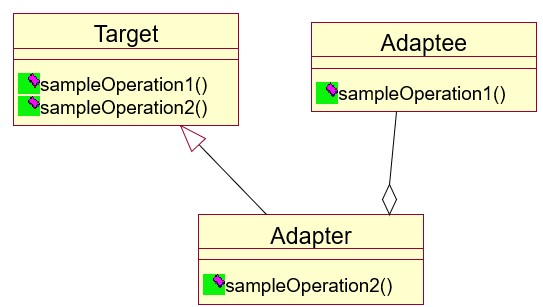
\includegraphics[width=0.50\textwidth]{20_3.jpg}
\end{figure}
%
\begin{lstlisting}[language=java]
public interface Target {
  void sampleOperation1();  // 源类有的方法
  void sampleOperation2();  // 源类没有的方法
}

public class Adaptee {
  public void sampleOperation1() {  }
}

public class Adapter implements Target {
  private Adaptee adaptee;
  public Adapter(Adaptee adaptee) {
    super();
    this.adaptee = adaptee;
  }
  public void sampleOperation1() {
    adaptee.sampleOperation1();
  }
  public void sampleOperation2() {
    // Write your code here
  }
}
\end{lstlisting}
%
适配器模式的目的是将接口不同而功能相同或相近的接口加以转换,这里面包括适配器角色补充了一个源角色没有的方法。

\textbf{对象型的适配器模式的效果}:
%
\begin{itemize}
  \item 一个适配器可以把多种不同的源适配到同一个目标。 即同一个适配器可以把源类和它的子类都适配到目标接口。
  \item 与类的适配器模式相比,要想替换源类的方法就不容易。如果一定要置换源类的一个或多个方法,就要先做一个源类的子类,将源类的方法替换,然后把源类的子类当作真正的源来适配。
  \item 虽然要想替换源类的方法不容易,但要想增加新的方法则很方便,而新增加的方法可适用于所有的源。
\end{itemize}
%
\textbf{什么情况下使用适配器模式}:
\begin{enumerate}
  \item 系统需要使用现有的类,而此类的接口不符合系统的需要。
  \item 想要建立一个可以重复使用的类.用于一些彼此之间没有太大关联的一些类,包括一些可能在将来引进的类一起工作,这些源类不一定有很复杂的接口。
\end{enumerate}
%
\subsection{Iterator和Enumeration}
在 JDK 1.0和1.1版本里没有java聚集(collection)的框架,
这一框架是在 JDK l.2版本中给出的。与此相对应,JDK1.0和1.1版本提供了enumeration接口,
而JDK 1.2版本给出了iterator接口。如果有很多的java代码是为老版本Java编译器写的,使用的是Enumeration,
现在想使用新版本编译器和新的Java聚集库包的话,需要将已有代码的Iterator 接口换成Enumeration接口.
因为Java聚集要求Iterator接口,这样才能使已有的代码可以使用新版本的聚集对象。

\textbf{从Iterator到Enumeration的适配}:
适配器Itermeration使用了对象的适配器模式,将一个Iterator对象封装在一个Enumeration类的具体类里。如下图所示:
%
\begin{figure}[H]
  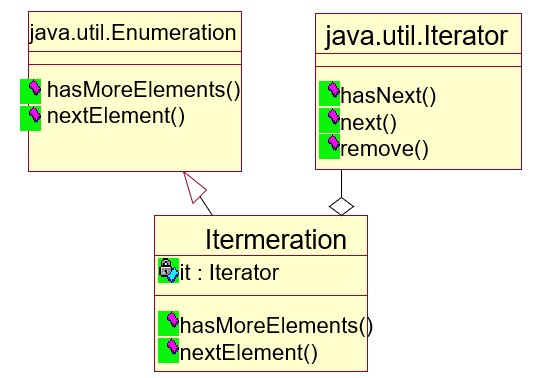
\includegraphics[width=0.50\textwidth]{20_4.jpg}
\end{figure}
%
\begin{lstlisting}[language=java]
import java.util.Enumeration;
import java.util.Iterator;
import java.util.NoSuchElementException;
public class Itermeration implements Enumeration {
  private Iterator it;
  public Itermeration(Iterator it) {
    this.it = it;
  }
  public boolean hasMoreElements() {
    return it.hasNext();
  }
  public Object nextElement() throws NoSuchElementException {
    return it.next();
  }
}
\end{lstlisting}
%
\textbf{从Enumeration到Iterator的适配}:
Enuterator使用了对象的适配器模式将Enumeration接口适配到Iterator接口。如下图所示:
%
\begin{figure}[H]
  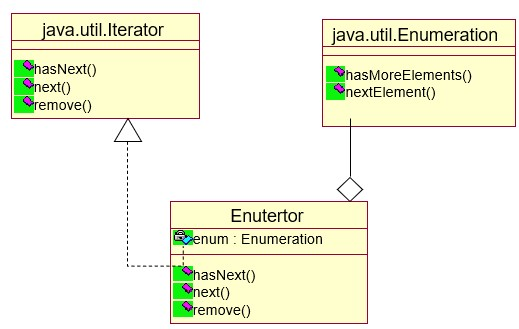
\includegraphics[width=0.50\textwidth]{20_5.jpg}
\end{figure}
%
\begin{lstlisting}[language=java]
import java.util.Enumeration;
import java.util.Iterator;
import java.util.NoSuchElementException;
public class Enuterator implements Iterator {
  private Enumeration enum;
  public Enuterator(Enumeration enum) { this.enum = enum; }
  public boolean hasNext() { return enum.hasMoreElements(); }
  public Object next() throws NoSuchElementException {
    return enum.nextElement();
  }
  public void remove() {
    throw new UnsupportedOperationException();
  }
}
\end{lstlisting}
%
\subsection{适配器模式在架构层次上的应用}
\begin{itemize}
  \item WINE是一个开源的免费软件,允许在linux环境里运行windows程序。 WINE提供了从Linux到Window图形界面的适配器。
  \item MKS Toolkit软件是一个为Windows系统设计的商业软件,它提供了C shell、Korn shell、Perl以及多种UNIX命令的解释器。在安装了此软件之后,Windows的用户可以在自己的系统上使用Unix的C Shell和Korn shell指令集合,以及如ls、vi、grep等的unix命令。也就是说MKS Toolkit提供了UNIX命令集从UNIX到windows的适配,是一种命令集层次上的适配器模式。
  \item JDBC驱动软件与适配器模式:JDBC给出一个客户端的通用界面。每一个数据库引擎的JDBC驱动软件都是一个介于JDBC接口和数据库引擎之间的适配器软件。
  \item 抽象的JDBC接口和各个数据库引擎的API之间都需要相应的适配器软件,即为各个数据库引擎准备的驱动软件。
\end{itemize}
\end{document}
